\documentclass[12pt, titlepage, oneside]{article}

\usepackage[margin=0.5in]{geometry}

\usepackage{siunitx, booktabs, amsmath, enumitem, pdfpages,mathrsfs,tabularx,caption, graphicx, pgfplots, textcomp,wrapfig, commath, svg}

\usepackage{amssymb}

\usepackage{parskip}

\usepackage[siunitx]{circuitikz}
\sisetup{detect-weight=true, detect-family=true}

\setlength\parindent{0pt}

\let\oldhat\hat
\let\oldvec\vec
\newcommand{\cross}{\bm{\times}}
\renewcommand{\hat}[1]{\oldhat{\mathbf{#1}}}

\usepackage{bm}
\renewcommand{\vec}[1]{\oldvec{\bm{#1}}}
\renewcommand{\hat}[1]{\oldhat{\bm{#1}}}
\renewcommand{\b}[1]{\textbf{#1}}

\newcommand{\de}[1]{\noindent\fbox{\parbox{\textwidth}{#1}}}

\newcommand{\be}{\begin{equation*}}
\newcommand{\ee}{\end{equation*}}

\begin{document}
	\setcounter{section}{9}
	\setcounter{page}{26}
 
    \section{Normal Distribution}

    Described with two parameters $\mu$ and $\sigma$, the \b{normal distribution} is denoted as $X \thicksim N(\mu, \sigma^2)$. The probability density function of a normal distribution is given by
    \begin{align}
      f(x) = \dfrac{1}{\sigma \sqrt{2 \pi}}\exp \Bigg(\,\dfrac{-1}{2}\bigg(\dfrac{x-\mu}{\sigma}\bigg)^2\Bigg)
    \end{align}

    For a normal distribution, $\sigma$ has a very precise meaning of spread of the distribution. There is a rule called ``68-95-99.7\%'' which specifies how much probability there is between certain multiplicities of $\sigma$ from the mean $\mu$
    \begin{align*}
      P( \mu - \sigma < X < \mu + \sigma) &= 0.68 \\
      P( \mu - 2\sigma < X < \mu + 2\sigma) &= 0.95\\
      P( \mu - 3\sigma < X < \mu + 3\sigma) &= 0.997
      \end{align*}
      So the effective width of $X$ is 6$\sigma$.

      \subsection{Standard Normal and Normal Table}
      Recall the probabilities for continuous random variables are obtained from areas under the p.d.f curve which require integration to get the c.d.f ($P(a < X \leq b) = P(b) - P(a)$). For the normal distribution there is no analytic formula for $F(x)$ and it requires numerical integration, that is areas obtained by tables or software.

      Table 3 in the appendix and attached to this note is the special case for $\mu = 0$ and $\sigma= 1$, this special case is called the standard normal distribution denoted by $Z \thicksim N(0,1)$. The notation for the standard normal p.d.f is $\phi(z)$, c.d.f $\Phi(z)$. In table 3 we have values for $\Phi(z) \equiv P(Z \leq z)$ for $-3.9 \leq z \leq 3.9$.

      To use table 3, find the first decimal of $z$ on the left most column, then find the second decimal on the top row. 
      
      \de{
        \b{Example 4.11} Find $P(Z > 1.26)$, $P(Z > 0.86)$, and $P(-1.25 < Z < 0.37)$
        \\

        \b{Ans.}
        \begin{align*}
          P( Z > 1.26 ) = 1 - P(Z \leq 1.26) = 1- 0.896165 = 0.103835\\
          P( Z > 0.86 ) = 1 - \Phi(0.86) = 1 - 0.805106 = 0.194894\\
          P( -1.25 < Z < 0.37) = \Phi(0.37) - \Phi(-1.25)  =  0.644309 - 0.105650 = 0.538659
        \end{align*}
      }

      \subsection{Standardizing a Normal Random Variable}
      Suppose that $X$ is a normal random variable with $E(X) = \mu$ and $V(X) = \sigma^2$, that is $X \thicksim N(\mu, \sigma^2)$ then
      \begin{align*}
        Z \thicksim \frac{X - \mu}{\sigma}
      \end{align*}
      $Z$ is a normal random variable with $Z \thicksim N(0,1)$, that is $Z$ is a standard normal random variable.

      $Z$ is called $Z-score$ or $Z-value$. It converts $X$ into a dimensionless quantity (if it isn't already dimensionless) as the units in numerator and denominator cancel.

      Suppose that $X \thicksim N(\mu, \sigma^2)$ and you want to find $F(x) = P(X \leq x)$. We write
      \begin{align}
        P(X \leq x) &= P\bigg( \frac{X - \mu}{\sigma} \leq \frac{x - \mu}{\sigma} \bigg)\\[2mm]
                    &= P\bigg(Z \leq \frac{x-\mu}{\sigma}\bigg)
      \end{align}
      So to find Normal probabilities or areas over a specified region, standardize the region to convert to a standard normal distribution and use table 3.

      \de{ \b{Example 4.13} Given $X \thicksim N(10,4)$, find $P(X > 13)$
        \begin{align*}
          P(X > 13) = 1 - P\bigg(\frac{X - \mu}{\sigma} \leq \frac{13 - 10}{2}\bigg) &= 1 - P(X \leq 1.5)\\
                                                                                     &= 1 - 0.933193 = 0.06681
          \end{align*}
        
        }

        \de{
          \b{Example 4.15 } Assume that in the detection of a digital signal, the background noise follows a normal distribution with a mean of $0$ volts and a standard deviation of $0.45$ volts. The system assumes a digital 1 has been transmitted with the voltage exceeds $0.9$. What is the probability of detecting a digital signal 1 when none was sent?
          \\

          \b{Ans.} Let the random variable $N$ denote the noise voltage. The requested probability is
          \begin{align*}
            P(N > 0.9) = P\bigg(\frac{N}{0.45} > \frac{0.9}{0.45} \bigg) = P(Z > 2) = 1-P(Z \leq 2) = 0.02275
          \end{align*}
          This is the probability of a false positive. A false negative is when a signal but was not received (aka. What is the probability the signal was lower than the noise).
          \\

          Suppose  that $X \thicksim N(0,0.45^2)$ is pure noise. Find a symmetric interval about 0 that would contain $99\%$ of all possible observations. In other words, we want
          \begin{align*}
            P(-x \leq X \leq x) &= P\bigg( \frac{-x-0}{0.45} \leq \frac{X-0}{0.45} \leq \frac{x-0}{0.45} \bigg)\\
                                &= P\bigg(\frac{-x}{0.45} \leq Z \leq \frac{x}{0.45} \bigg)\\
                                &= 0.99
          \end{align*}
          This examples utilize the standard normal tables in reverse. We are looking for an interval $(-z,z)$ under the $Z$ curve which should equal $0.99$. So the area outside $(-z,z)$ is $0.01$ which should be split into two equal areas as by symmetry the $0.01$ should be the area on either side of our distribution. So the tails of our distribution is $0.005$. Therefore, if we look at the area from $(-\infty, z)$ we should have $0.005 + 0.99 = 0.995$. We now look for a $z$ value such that $P(Z \leq z) = 0.995$, and we find $z = 2.58$. Now we solve for $x$
          \begin{align*}
            \frac{x}{0.45} &= 2.58\\
            x &= 1.161
            \end{align*}
          }

          \subsection{Percentiles}
          Let $0 < p < 1$. The $100^{th}$ percentile of $X$ is a point $x_p$ such that
          \begin{align}
            P(X \leq x_p) \equiv F(x_p) = p
          \end{align}
          Which means the area to the left of $x_p$ equals $p$

          \subsubsection{Percentile of Standard Normal $Z$}

          In statistics, for Normal Random Variables it is customary to refer to percentiles by area $\alpha \equiv 1-p$ to the right of $x_p$. Thus for $0 < \alpha < 1$ let $z_{\alpha} = P(Z \geq \alpha)$ denote the $100(1-\alpha)^{th}$
          \begin{center}
            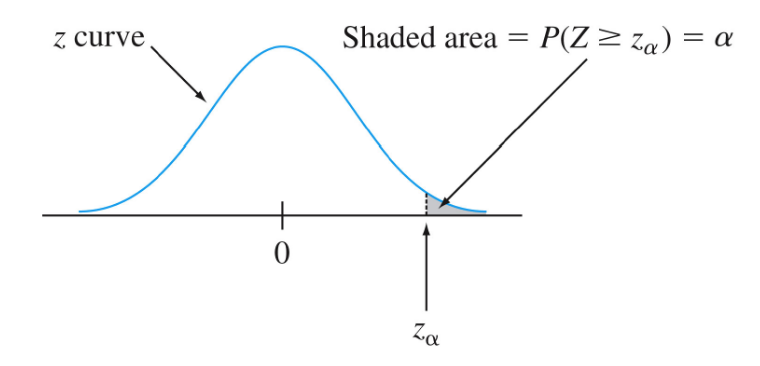
\includegraphics[scale=0.35]{1.png}
          \end{center}
          From $Z = \dfrac{X - \mu}{\sigma}$ we can cross multiply to get
          \begin{align}
            X = \mu + Z \sigma
          \end{align}
          $100p^{th}$ percentile of $X = \mu + \sigma (100p^{th})$ percentile of $Z$ or more symbolically
          \begin{align}
            x_p = \mu + \sigma z_{1-\alpha}
          \end{align}

          \de{
            \b{Example} Coffee is dispensed by a machine is $X \thicksim N(8, 0.30^2)$ ounces. What container size $c$ ensures that overflows occurs only $0.5\%$ of the time?
            \\

            \b{Ans.} Find $c$ so that $P(X > c) = 0.005$. Since $c$ requires to hold the $99.5^{th}$ percentile of coffee dispensed
            \begin{align*}
              c = 8 + 0.30(z_{1-\alpha})
            \end{align*}
            $z_{1-\alpha}$ is given by $\alpha = 1 - 0.005 = 0.995$ (Recall, $\alpha$ is the area to the right). So we are looking for $z_{0.005} = 2.58$.
            \begin{align*}
              c = 8 + 0.30(2.58) = 0.77
              \end{align*}
            A more easier way to pick $z_{1-\alpha}$ is to see that $c$ must cover $99.5$ percent. Thus we must find a $\Phi(z) = 0.995$
          }
         
\end{document}